\documentclass[12pt]{article}
\usepackage{listings}
\usepackage{amsmath}
\usepackage{amssymb}
\usepackage{array}
\usepackage{authblk}
\usepackage{bm}
\usepackage{booktabs}
\usepackage{a4}
\usepackage{calc}
\usepackage{caption}
% \usepackage{ctex} %不想要中文就注释掉
\usepackage{fancyhdr}
\usepackage{graphicx}
\usepackage{hyperref}
\usepackage{ifthen}
\usepackage{longtable}
\usepackage{multicol}
\usepackage{ntheorem}
\usepackage{paralist}
\usepackage{titlesec}
\usepackage{fancyvrb}
\usepackage{fontspec}
\usepackage{geometry}
\usepackage{titletoc}
\usepackage{xcolor}
% \usepackage{xeCJK}
\usepackage{fontspec}
\usepackage{lastpage}
\setmainfont{Times New Roman}

\makeatletter
\newcommand\dlmu[2][4cm]{\hskip1pt\underline{\hb@xt@ #1{\hss#2\hss}}\hskip3pt}
\makeatother

\newenvironment{cmd}{\fontfamily{Arial}\selectfont}

\begin{document}
\begin{titlepage}
    \begin{center}
        {~}\\[3cm]
        % {\Huge2021数学建模美国赛电子科技大学\\模拟赛}\\[5cm]
        % {\huge2021数学建模美国赛电子科技大学模拟赛}\\
        % 队号:\dlmu[7cm]{H275}\\[2cm]
        % 队员:\dlmu[7cm]{王大杨~陈麒至~王泽寰}\\[5cm]
        % \today
        % \begin{cmd}
        \Huge\textbf{Holiday Life: How do College Students Choose Part-time Jobs during Holidays}\\[5cm]
        % \end{cmd}
        \large Dayang Wang,~Qizhi chen,~Zehuan Wang\\[4cm]
        \small{\today}
        % \maketitle
    \end{center}
\end{titlepage}

\begin{abstract}
%-----------------------------------------
% 在这篇文章中,我们从多方面入手,考虑了可能影响大学生选择兼职的各个因素,基于大量的数据利用最小二乘法拟合出兼职工作满意度期望同收入、工作条件和工作类型等之间的关系,并在合理假设的基础上利用层次分析法作出基于个人不同偏好下对已知可选工作最优的选择方案,以此来帮助大学生合理选择兼职工作。
In this article, we start from many aspects, and considering various factors that may affect college students' choices on part-time jobs, based on a large amount of data using ordinary least squares fitting of the part-time job satisfaction expectations with income, working conditions, and the relationship between the type of work and so on, and on the basis of the hypothesis of rational use of analytic hierarchy process (AHP) to make the choice of the optimal solution based on personal preferences on known optional work , in order to help students choose a part-time job.
~~\paragraph*{Key~words:}ordinary least squares,~trust-region,~LM,~optimization method,\\~hypothetico-deductive-method
\end{abstract}

\pagestyle{fancy}\fancyhf{}\fancyhead[C]{Team H275,~Problem A}\rfoot{Page \thepage \hspace{1pt} of \pageref{LastPage}}\setcounter{page}{1} %用来将正文第一的页码设为1.
\tableofcontents\thispagestyle{empty}\newpage

\setcounter{page}{1} %用来将正文第一的页码设为1.
\section{Introduction}
\subsection{Background}
%众所周知,大学生活相对而言更加考验学生们对自我时间的管理和应用能力,同时,大学也是学生们完全进入社会前增长见识,体验生活的一段宝贵时光。因此,许多大学生们选择在生活学习压力相对较小的假期进行课外兼职,以此开拓自己的眼界并增长社会阅历。然而,许多大学生在面对大量的兼职招聘信息时常常感到茫然,不知道应当如何选择一份适合自己的兼职工作。为此,我们决定作出一个模型,来帮助大学生们从已知的工作中选择最适合自己的
~~As is known to all, college life relatively tests students' ability to manage and apply their own time. Meanwhile, college life is also a precious time for students to increase their knowledge and experience life before they fully enter the society. Therefore, many college students choose to take extra-curricular part-time jobs during the holidays when the pressure of life and study is relatively low, so as to broaden their horizons and increase their social experience. However, many college students often feel at a loss when faced with a large number of part-time job postings and do not know how to choose a part-time job that suits them. To this end, we decided to develop a model to help college students choose the job that best suits them from the known jobs.
%-----------------------------------------------------
\subsection{Restatement of the Problem}
~~
%我们要帮助大学生选择最适合他们的工作。通常,影响最大的因素为工作收入、通勤时间、工作时长、工作时间段和工作安排的灵活性,以及其他硬性要求和用户的个人偏好。为此,我们需要综合上述信息作出最好的判断,并筛选出值得推荐的工作反馈给用户
We should help college students choose the job that suits them best. In general, the most influential factors are income from work, commuting time, working hours, working period, flexibility of work schedule and working environment, as well as other rigid requirements and personal preferences of users. Therefore, we need to make the best judgment based on the above information, and filter out the work worthy of recommendation to feedback to users.


% \newpage
\section{Analysis of the Problem}
%显然,上述影响因素具有不同的性质。
%一方面,对于某些变量,不同人对其的期望往往具有相同的趋势,但对其他的,不同人之间的选择往往有很大差异且互不相关。例如,人们几乎都希望获得更高的收入,花费更少的时间,拥有更好的工作环境;但是不同人对于各个职业的偏好并不总从上述规律,有的人喜欢文职类工作,而有的人则更倾向于户外工作。
%另一方面,有些变量易于量化或按照评级的方式进行近似量化,而有些变量则难以量化。例如,收入、工作时间等可以轻易用数值来表示,但兼职工作的类型(如家教、收银员)等则难以量化为具体的数值或进行评级。
~~Obviously, the above factors have different properties:
\begin{itemize}
    \item On the one hand, for some variables, the expectations of different people tend to have the same trend, but for others, the choices between different people tend to be very different and unrelated. For example, people almost always want to earn more money, spend less time and have a better working environment. But the pattern does not always follow. Some people prefer civilian work, while others prefer outdoor work;
    \item On the other hand, some variables are easy to quantify or approximate in the manner of ratings, while others are difficult to quantify. For example, income, hours worked, etc. can easily be expressed in numerical terms, but the type of part-time job (such as tutor, cashier) is difficult to quantify or rate.
\end{itemize}
%基于上述情况,我们可以对这些部分分开进行处理。我们发现无法量化的地方恰好也是不同用户的选择出现较大不同的地方,因此我们考虑下面的解决方案:
~~Based on the above situation, we can treat these parts separately. We found that the unquantifiable areas also happened to be places where the choices of different users were quite different, so we considered the following solution:
~~\begin{itemize}
    %对于不能数值化的数据,由用户自行进行选择或排除(可选择或排除0项,一项或多项),根据用户的选择限定可考虑的兼职工作范围
    \item For data that cannot be quantified, users can select or exclude (0 items, one or more items can be selected or excluded) by themselves, and limit the range of part-time jobs that can be considered according to the user's choice;
    %对于可以数值化的数据,由程序处理,根据给定的数据(例如这份工作的收入、工作时间等)自动生成某一项的得分。用户根据自己的喜好对不同项施加一定的权重后,各项带权值相加的到可数值话的最后分数。分数越高,越值得推荐。 
    \item For data that can be quantified, the program processes and automatically generates a score based on the given data (such as the income of the job, hours worked, etc.). After the user applies certain weights to different items according to his/her preferences, the final score of each item with weights added up to numerable words. The higher the score, the better the recommendation.
\end{itemize}
%因此,在用户自行选择限制条件(当然,用户也可以无视限制条件,即通过全选或全不选的方式)的基础上,进行个人偏好评估,由评估结果生成各项对应的权值,结合程序自动生成的各项得分带权相加并排序。在此过程中,除去自行选择环节,其他过程具体实现对用户隐藏,只给出推荐结果。
~~Therefore, on the basis of the user's self-selection of the restrictions (of course, the user can ignore the restrictions by choosing all or none), the individual preference evaluation is carried out, and the corresponding weights are generated from the evaluation results. In combination with the automatically generated scores with weights, the weights are added and sorted. In this process, the self-selection link is removed, and the other processes are specifically hidden from users, and only the recommended results are given.


% \newpage
\section{Symbols}
    \begin{table}[!htp]
    % \caption{Symbols}  
    \begin{tabular*}{15cm}{ll}
            \hline
            Definitions & Description\\
            \hline
            $A$      & Weighted row vector\\%权重行向量\\
            $a_i$ & The weights of the terms in A,~i=1,2,3,4,~$\sum_{i=1}^{4}a_i=100$\\%A中各项的权值
            $B_{0}$      & A custom matrix B, with each row representing a job and each column\\ & representing a property of the corresponding job\\%自定义的矩阵B,每行代表一个工作,每列代表对应工作的一项性质
            $B$ & Modified matrix $B_{0}$\\%B0修正后的矩阵
            $b_{ij}$ & The element at row i, column j in matrix B\\
            $\Delta b_{j}$ & The average difference of element in column j in B\\%B中第j列的元素平均差值
            $r$ & The correlation coefficient\\
            $\bar{x}$ & The average salary for each job\\%各个工作对应的工资平均值
            $\bar{y}$ & The average working hours for each job\\%各个工作对应工作时长平均值
            $t_{m}$ & The working time for job m\\
            $s_{m}$ & The salary for job m\\
            $e_{m}$ & The working environment of job m\\
            $f_{m}$ & The flexibility of job m\\
            slm & Shorthand of salesman\\
            wtr & Shorthand of waiter\\
            tch & Shorthand of private teacher\\
            dlv & Shorthand of delivery man\\
            wkr & Shorthand of labor\\
            hrw & Shorthand of hourly worker\\
            ntw & Shorthand of IT worker\\ 
    \end{tabular*}
\end{table}
\begin{table}
    \begin{tabular*}{15cm}{ll}
        \hline
        Definitions & Description\\
        \hline
        slm & Shorthand of salesman\\
        wtr & Shorthand of waiter\\
        tch & Shorthand of private teacher\\
        dlv & Shorthand of delivery man\\
        wkr & Shorthand of labor\\
        hrw & Shorthand of hourly worker\\
        ntw & Shorthand of IT worker\\ 
    \end{tabular*}
\end{table}

\section{Simplifying Assumptions}
~~In order to simplify the problem, we make the following assumptions based on the actual situation:
~~
\begin{enumerate}
    \item No accidents due to force majeure, such as earthquake and other natural disasters;
    \item All actions are legal;
    \item The source of data is real,universal and reliable;
    \item The data are from domestic statistics of China (excluding Hong Kong, Macao and Taiwan) and are only valid within China;
    \item Domestic and international situation remained stable;
    \item Everyone can apply for more than one job at a time, and they don't interfere with each other;
    \item There are individual differences in users' preferences;
    \item The users' physical and psychological conditions are normal, or the users are clearly aware of their own diseases and refuse to choose to work in an unsafe or unhealthy way that may endanger their life and body;
    \item Gender doesn't matter.
\end{enumerate}
%=================================================================================================================
\section{Data Processing}
~~
%通过问卷调查【数据来自电子科技大学调查问卷和自研问卷】和随机采访路人,我们认为可以将大学生们常用的兼职分为七类:销售员(slm),服务员(wtr),私人教师(tch),快递外卖员(dlv),工人(wkr),小时工(hrw)和IT工作者(ntw),因为这几类占据了绝大多数人的选择;可量化影响因素分为收入s、工作时间t、工作环境e、和工作灵活性f,因为它们在问卷中被选择的概率远远大于其他项。因此,我们采取“从一般到特殊”的思想,关注影响最大的关键因素,利用假说演绎法来构造一个可以相对精确推荐兼职工作的模型:
Through the questionnaire survey\footnote[1]{The data were obtained from the questionnaires in appendix A} and random interviews with passers-by, we think that college students part-time commonly used can be divided into seven categories: the salesman (slm), the waiter (wtr), private teachers (tch), express delivery agent (dlv), workers (wkr), hourly workers (hrw), and IT workers (ntw), because of this a few class occupied the vast majority of people choice; The quantifiable influencing factors are income S, working time T, working environment E, and working flexibility F, because they are far more likely to be selected in the questionnaire\footnote[1]{From the questionnaire in appendix B} than other items. Therefore, we adopt the idea of "from general to special", focus on the most influential key factors, and use the hypothesis deduction method to construct a model that can recommend part-time jobs relatively accurately:
\begin{enumerate}
    %首先利用常见的几类工作的平均情况作为参考,得出兼职工作收入s、工作时间t、工作环境e和工作灵活性f的平均值
    \item Firstly, the average situation of several kinds of representative jobs are used as a reference to obtain a universally applicable determination method;
    \item To get a more accurate result, we should quantify the degree of superiority and inferiority of the work, denoted as W;%为了得到更加准确的结果,我们应当对该工作的优劣程度进行量化,记为W
    \item Unitalize $s, t, e, f,$ and replace absolute values with relativistic ones. The purpose of unitization is to ensure that the same deviation from the mean is equivalent to the same value among different influencing factors. When the user applies the same weight to all four factors, the job with the highest average overall ranking of all four factors should be selected. In other words, the user has the right to directly choose the weight that he is willing to pay for each item and the result is not affected by the absolute value of an item. When the four rankings are the same, the user's weight allocation directly determines the overall rating score of the job%将s,t,e,f单位化,用相对化数值代替绝对数值。单位化的目的是保证在不同影响因素中,相对于均值的偏移程度相同等价于他们的数值相同。当用户对这四个因素施加同样的权重时,应当选择到四项因素平均综合排名最高的工作。也就是说,用户有权直接选择愿意付给每一项的权重且结果不会因为某一项的绝对数值大小而受影响。当这四项各自的排名相同时,用户的权重分配直接决定了工作的总评得分
    \item As for the weight input by the user, we generally want to work for a shorter time, so we set the weight corresponding to T as the negative number input by the user;%对于用户输入的权值,由于我们普遍希望工作时间更短,故我们将t对应的权值置为用户输入的相反数
    \item Through analysis and calculation, the most possible functional relationship between W and all the data is fitted, that is, W is approximate to... Function expression of s, t, e, f;%通过分析和计算,拟合出W和各项数据之间最可能的函数关系,即近似得到W关于........的函数表达
    \item In the following process, the real data obtained by sampling will be used for inspection and testing, and return to Step3 for further modification;%在后续过程中利用采样得到的真实数据进行检验和测试,并返回3进一步修正
    \item Put it into use.%投入应用
\end{enumerate}
%在具体细节实现上,我们首先结合统计数据【引用2】对写出矩阵B0.然后对B的每一列分别分别求取平均值,以平均值作为他们的基准,每一项和基准的比值作为这一个元素在B中的值。这样。我们就对s,t,e,f完成了单位化。
%
~~In the implementation of specific details, we first write the matrix $B_{0}$ based on the statistical data\footnote[2]{he data were obtained from the questionnaires in appendix A}.Then take the average of each column of $B_{0}$, and take the average as their benchmark, and the ratio of each term to the benchmark as the value of this element in $B$。Like this. We've just done the unitization of $s, t, e, f$. 

\section{Model and Solution}
~~In four known factors, the data from all work compensation and working hours in 58 recruitment website and where to comprehensive data extraction, with the data obtained in the average one for the unit, each factor and the difference of average income divided by average number plus one can get the factors to the corresponding type of work on the right, under the assumption that people are the average of shorter working hours, the greater the degree of be fond of, under the condition of our working hours income right is negative. For influence factors on the role of the selected type of work we have assumed the effect are same, so we work for the working environment and flexibility of the weight distribution based on the weight distribution of compensation, in considering the natural and social environment and the work is carried out under the risk, the type of work, we take the same ranking medium the reset to a type of work right take the weighted average poor, compensation based on ranking and subtract the mean values, the poor get working environment corresponding weights, in the same way, considering limitation of work, the work of the immobility of time, the preparation of the work conditions to evaluate work flexibility, commuter You get the weights. Column the final result into a matrix $B$\\%在四个已知影响因素中,均工作薪酬与工作时长所得数据在五八招聘网站以及去哪儿网中进行数据提取综合得到,以所得数据中平均数为单位一,每个因素和平均值的差值再除以平均值所得数加一即可得该因素作用到对应工种上的权,其中在假设人们均对平均工作时长越短则喜好度越高的情况下,我们的工作时长所得权为负数。对于影响因素在已选工种的作用上我们已假设效果均相同,因此我们对于工作环境和工作灵活性的权重分配建立在薪酬的权重分配基础上,在综合考虑工作地自然、社会环境以及工作风险下,我们对工种进行排名,同样取排名中等的工种权重置为一,取薪酬中权重极差进行平均,在排名基础上加减该极差平均值,得到工作环境对应权重,同理,考虑工作的限制性,工作时段的固定性,工作的准备阶段,通勤情况之后对工作灵活性进行评估,得到相应权重。将最后结果列成一个“工作”矩阵
~~\begin{table}[htp]
    \begin{tabular}{lllll}
                                   & s    & t   & e  & f \\
        \hline
    slm                       & 1.05  & -1.167 & 1     & 0.911 \\
    wtr                         & 0.628 & -0.743 & 1.089 & 1     \\
    tch                & 1.217 & -1.061 & 1.178 & 0.733 \\
    dlv                   & 1     & -1.061 & 0.911 & 1.089 \\
    wkr & 1.25  & -1.061 & 0.733 & 0.822 \\
    hrw                  & 1.05  & -1.061 & 0.822 & 1.267 \\
    ntw       & 0.783 & -0.849 & 1.267 & 1.178
    \end{tabular}
\end{table}
~~The first three in the collection table are entitled multiple choice questions, if the person who fills the form has a rigid requirement, can directly cancel some work, the last four is entitled the person who fills the form to cast weight, the person who fills the form for each factor emphasis is different, then the weight of cast is also different, the weight of cast determines the algorithm to give the recommended work. Multiply the work matrix with the data obtained from the collection table, and the data obtained will be the three most suitable jobs for the corresponding job type under the choice of the person who fills the table.\\%收集表中前三题为选择题,填表人若有硬性要求则可直接取消一些工作,后四题为填表人投权重,填表者对于每个因素的侧重点不同,则所投权重也不同,投的权重即确定了本算法给与推荐的工作.将工作矩阵与收集表所得数据所乘,得到数据即为对应工种在填表者的选择下最适合的三项工作。
~~After the model is obtained, it corresponds to any specific work that conforms to the user's choice. We only need to bring $s, t, e and f$ of this work into the above model framework to get its score. Only three with high recommendation scores are needed\\%得到模型后,对应任意符合用户选择的具体工作,我们只需要将该工作的s,t,e,f带入上述模型框架,就能得到其评分。只需推荐评分较高的三个即可


\section{Validation}
~~
%我们虚拟了10个大学生来选择他们职业,以此来检验模型的正确性和可行性。经过检验,模型复合我们的预期
The correlation between each factor and the result was tested, and 4 columns in the work matrix were extracted. Set four vectors A, B, C and D, A= salary; B= working hours; C= Working environment; D= flexibility of work, set W= calculation result matrix, conduct three-dimensional fitting analysis of W and ABCD in pairs, $r$ are both above 0.9 except for one which is 0.8, as the figures shown below. Therefore, W and ABCD have a high joint correlation, and it is feasible to assign the weight of ABCD in the hypothesis.
\begin{figure}[htbp]
    \centering
    % \subfigure[pic1.]
    {
    \begin{minipage}[t]{0.3\linewidth}
    \centering
    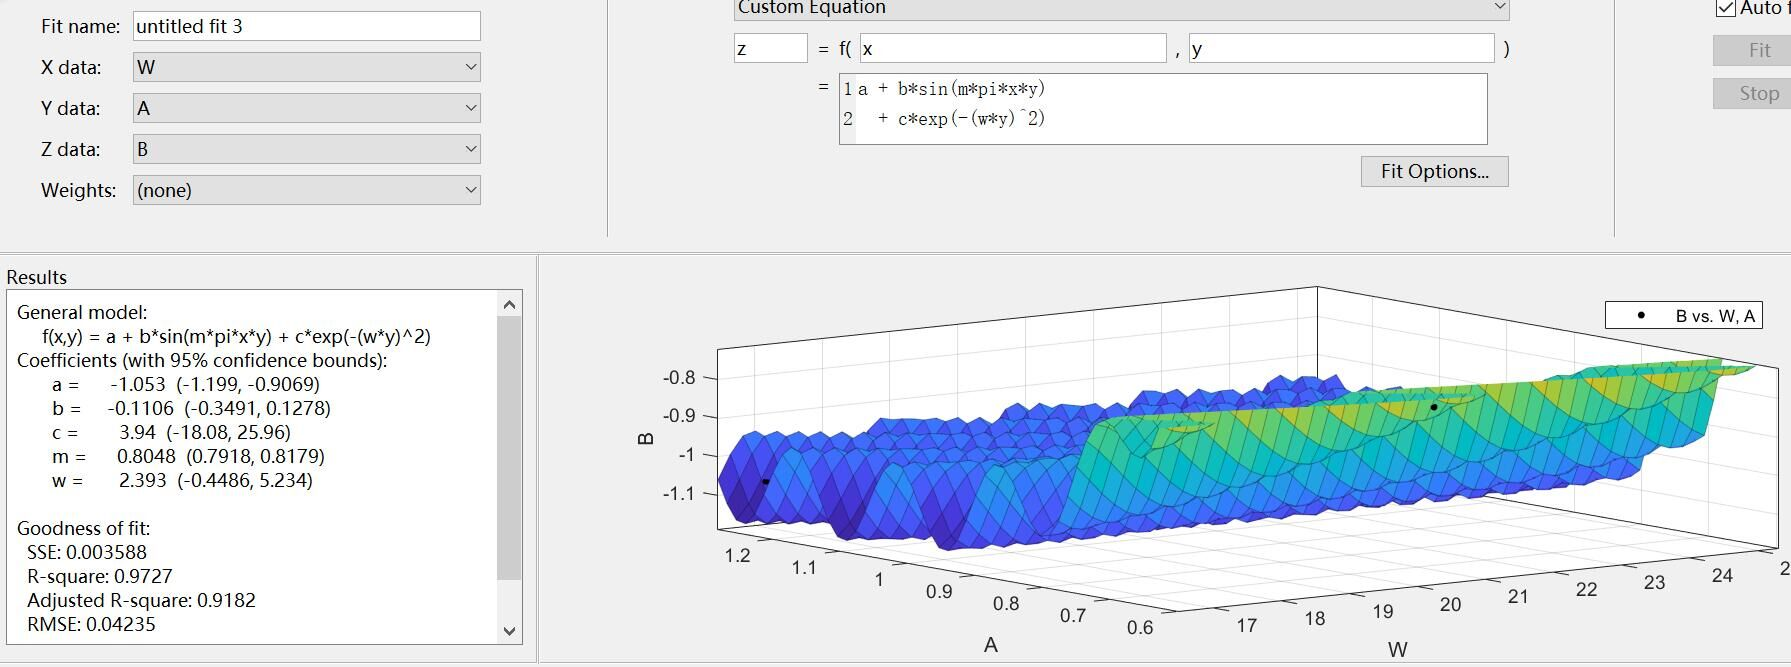
\includegraphics[width=1.7in]{figure/pict1.jpg}
    %\caption{fig1}
    \end{minipage}%
    }%
    % \subfigure[pic2.]
    {
    \begin{minipage}[t]{0.3\linewidth}
    \centering
    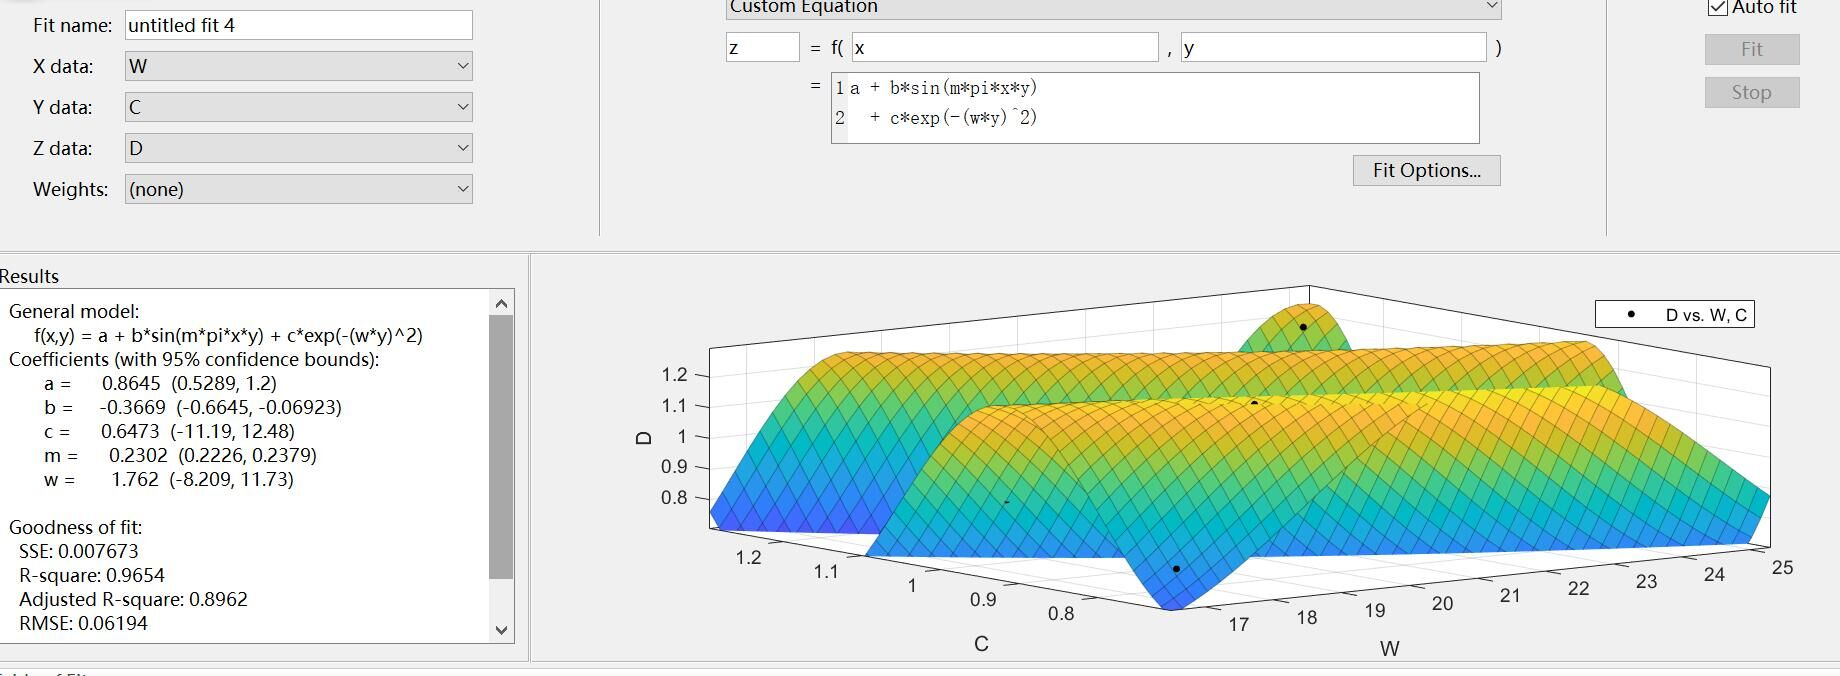
\includegraphics[width=1.7in]{figure/pict2.jpg}
    %\caption{fig2}
    \end{minipage}%
    }%
                     %这个回车键很重要 \quad也可以
    % \subfigure[pic3.]
    {
    \begin{minipage}[t]{0.3\linewidth}
    \centering
    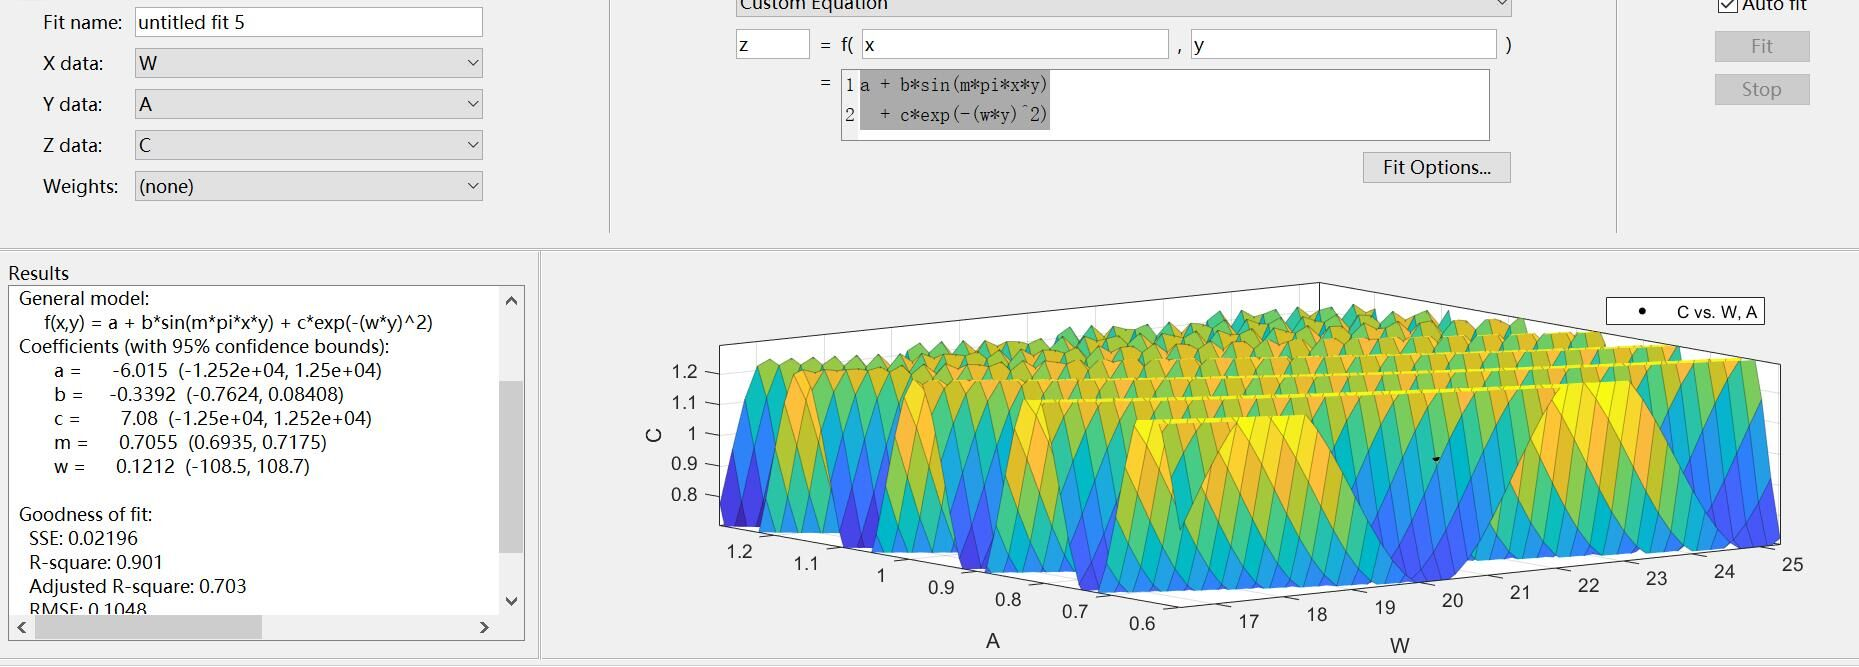
\includegraphics[width=1.7in]{figure/pict3.jpg}
    %\caption{fig2}
    \end{minipage}
    }%
    % \subfigure[pic4.]
    {
    \begin{minipage}[t]{0.3\linewidth}
    \centering
    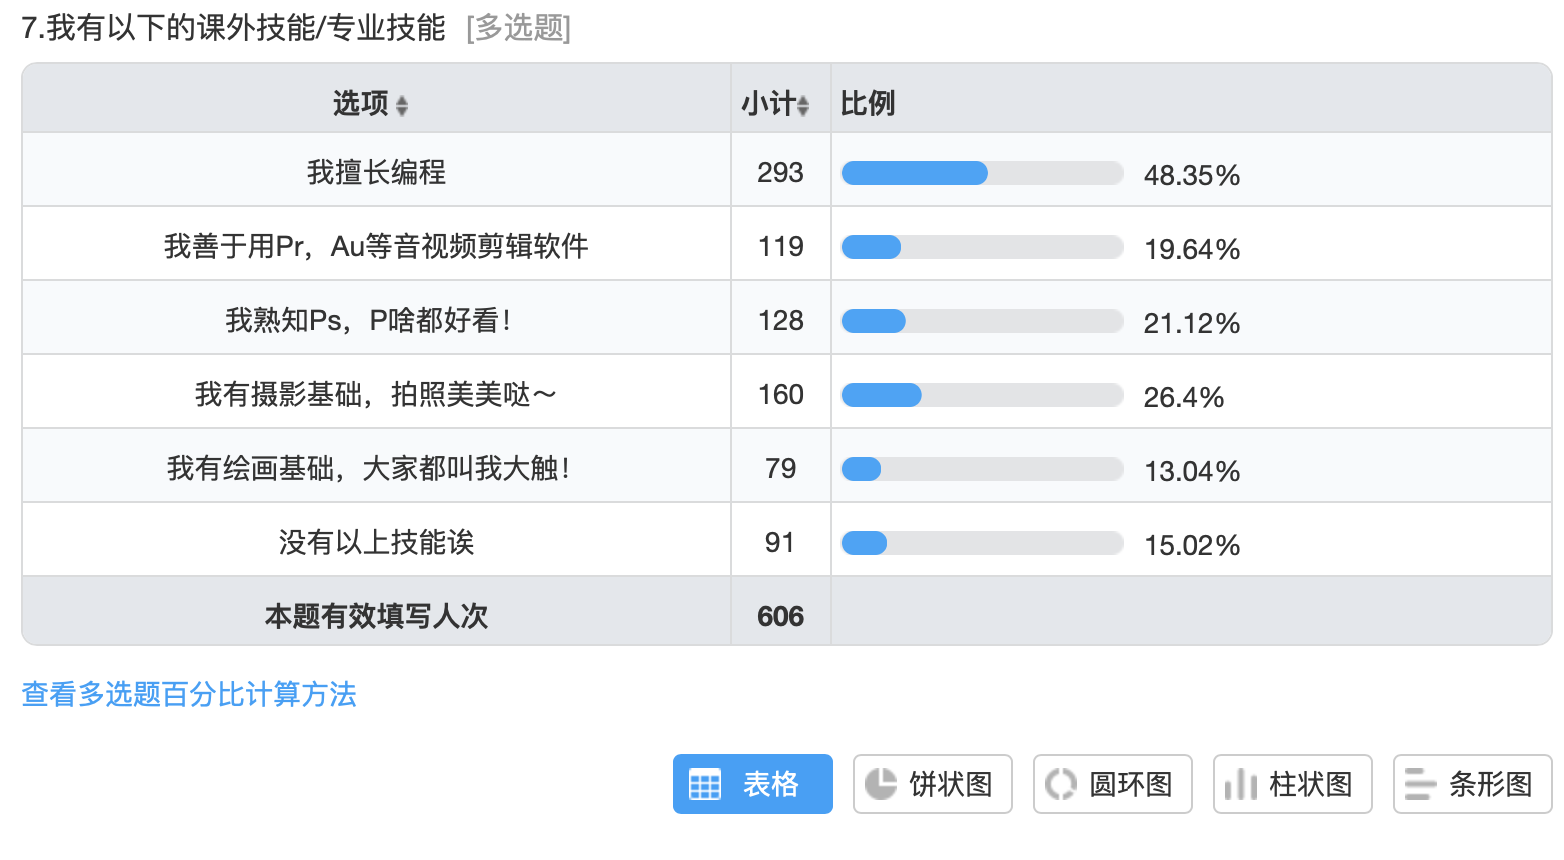
\includegraphics[width=1.7in]{figure/pic4.png}
    %\caption{fig2}
    \end{minipage}
    }%
    {
    \begin{minipage}[t]{0.3\linewidth}
    \centering
    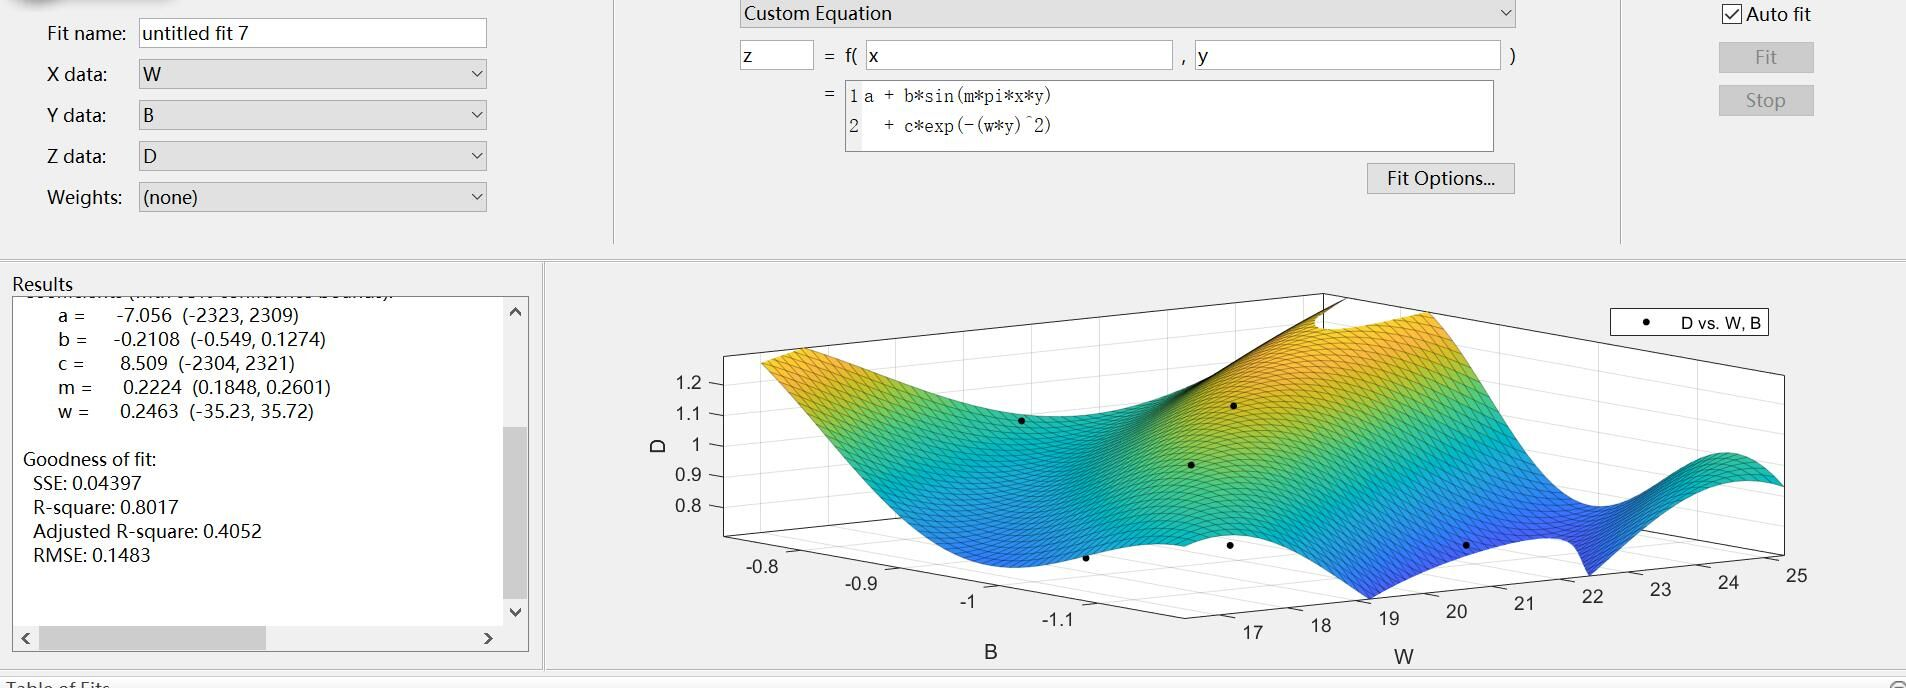
\includegraphics[width=1.7in]{figure/pict5.jpg}
    %\caption{fig2}
    \end{minipage}
    }
    {
    \begin{minipage}[t]{0.3\linewidth}
    \centering
    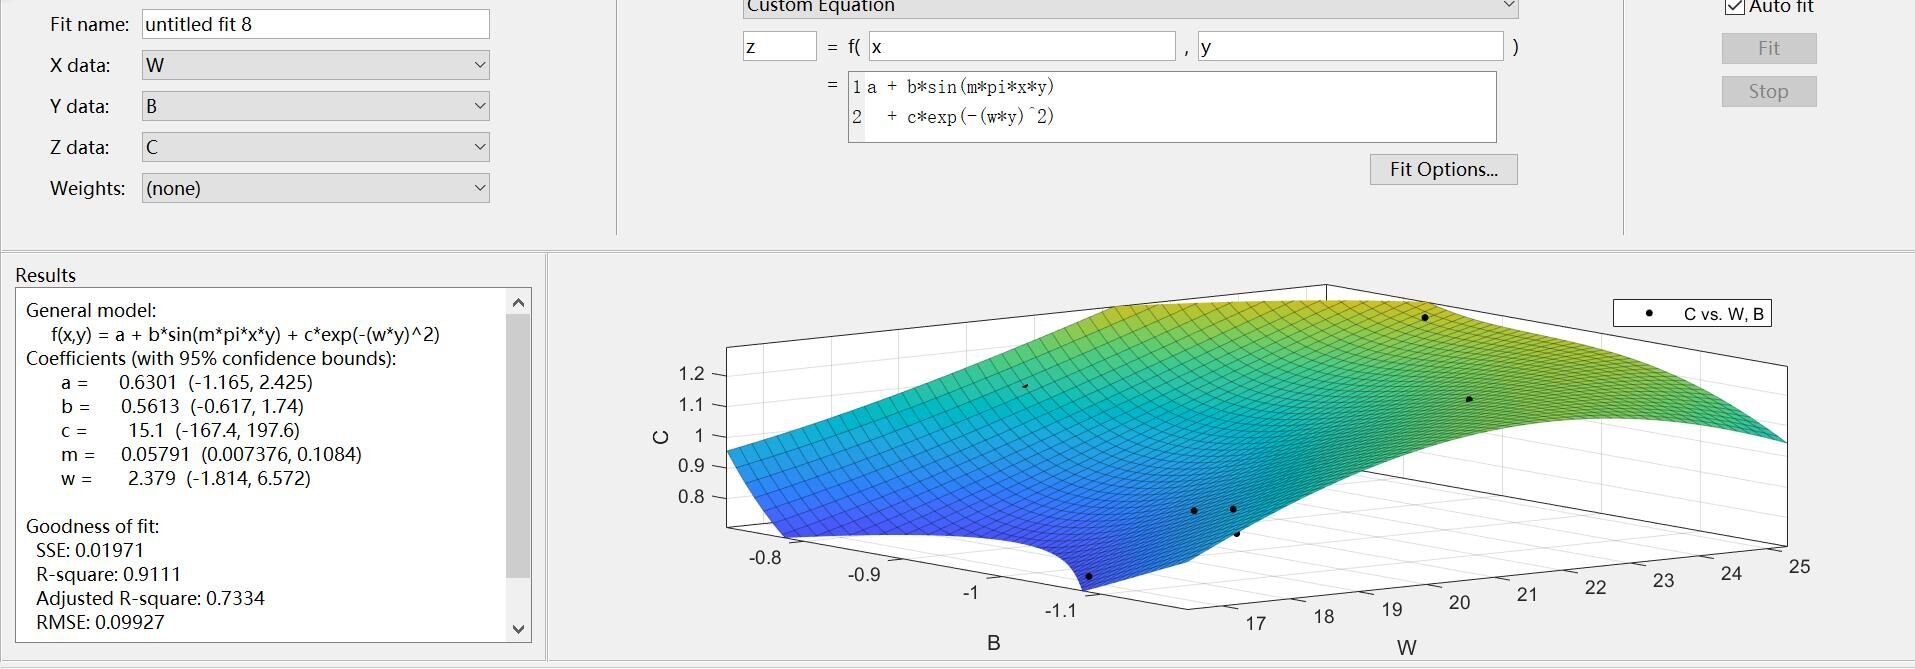
\includegraphics[width=1.7in]{figure/pict6.jpg}
    %\caption{fig2}
    \end{minipage}
    }
    
    % \centering
    % \caption{ pics}
    \end{figure}
We also simulated 10 college students to choose their careers to test the correctness and feasibility of the model.Upon examination, the model met our expectations\footnote[1]{See appendix D for results}.


\section{Application}
~~In order to simplify the user's difficulty and ensure the accuracy of the program, we only need to complete the following content as shown in the figure below%为了简化用户使用难度的同时保证程序的准确性,我们只需要完成如下图所示内容即可
\begin{figure}[!htbp]
    \centering
    % \subfigure[pic1.]
    {
    \begin{minipage}[t]{0.3\linewidth}
    \centering
    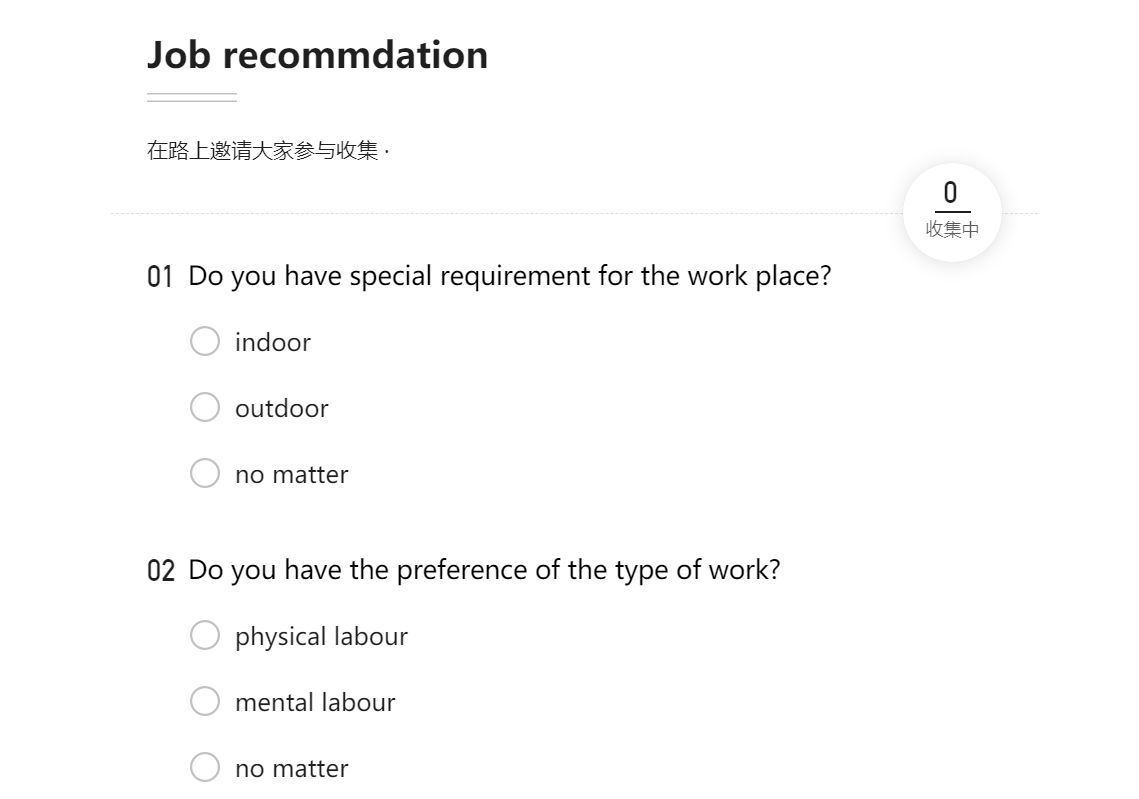
\includegraphics[width=1.7in]{figure/t1.png}
    %\caption{fig1}
    \end{minipage}%
    }%
    % \subfigure[pic2.]
    {
    \begin{minipage}[t]{0.3\linewidth}
    \centering
    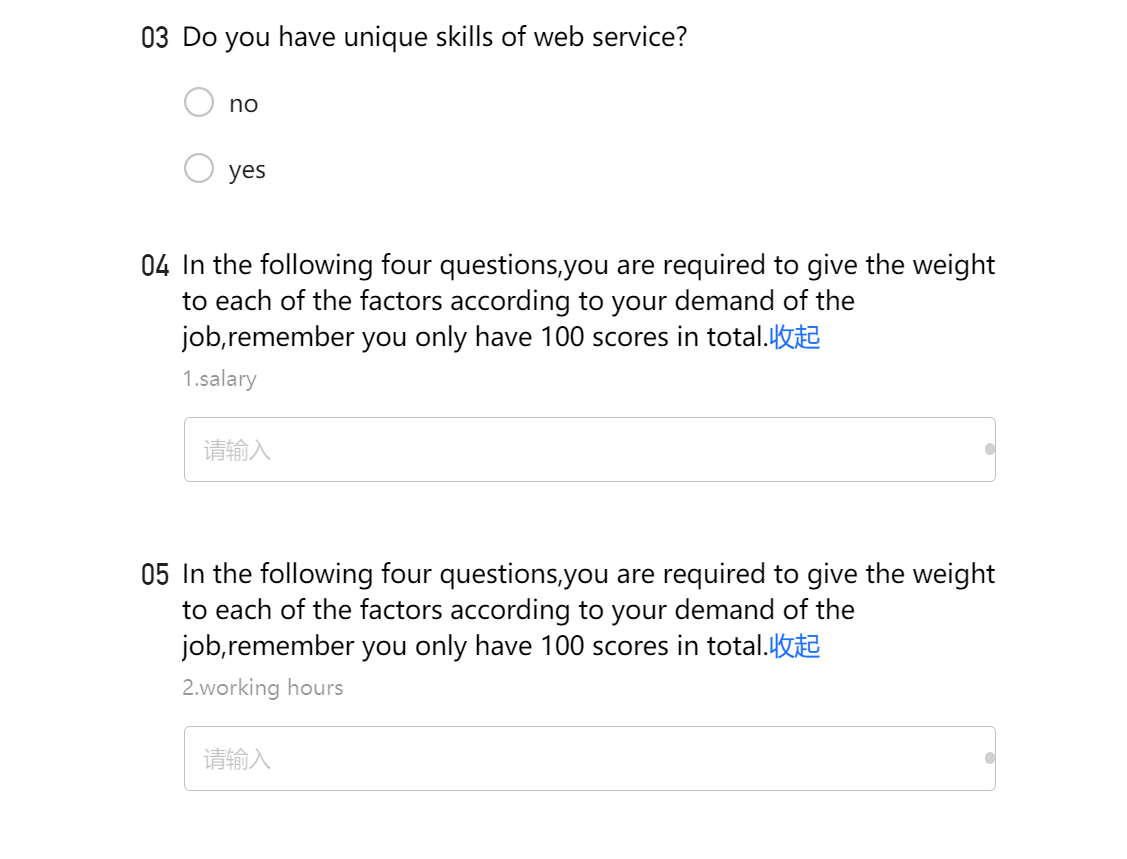
\includegraphics[width=1.7in]{figure/t2.png}
    %\caption{fig2}
    \end{minipage}%
    }%
                     %这个回车键很重要 \quad也可以
    % \subfigure[pic3.]
    {
    \begin{minipage}[t]{0.3\linewidth}
    \centering
    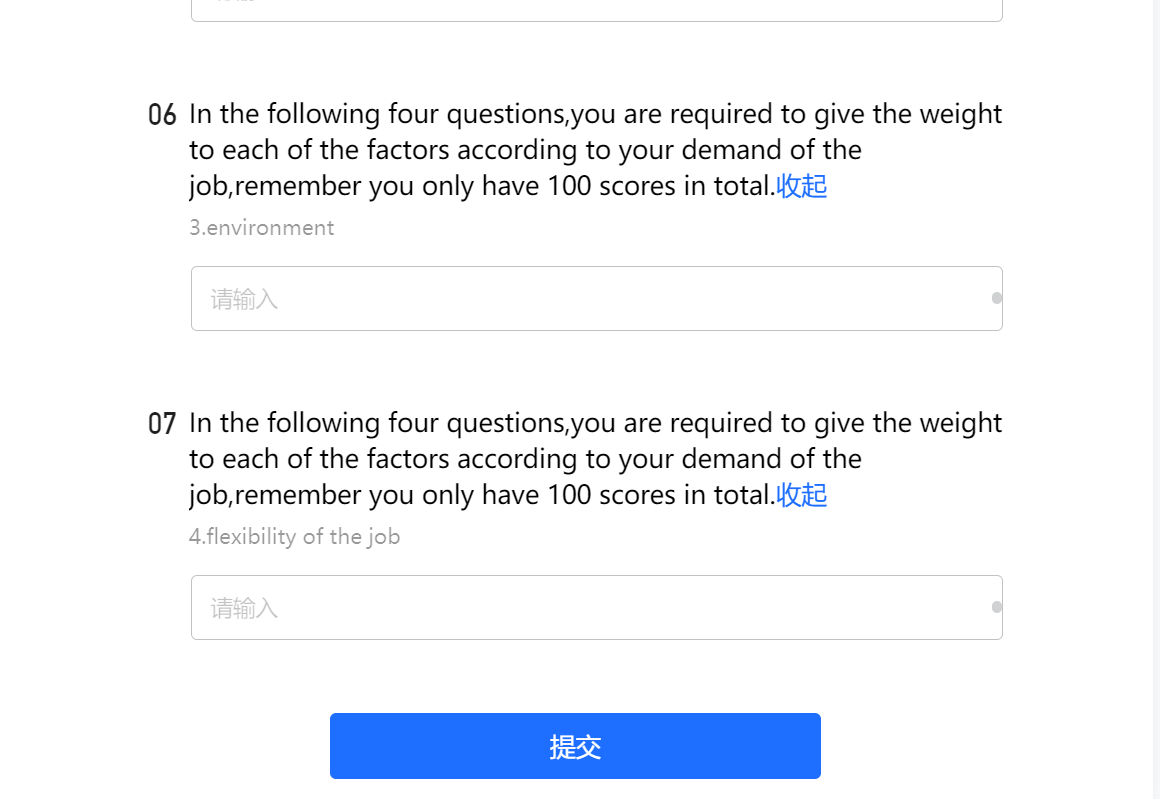
\includegraphics[width=1.7in]{figure/t3.png}
    %\caption{fig2}
    \end{minipage}
    }%
    % \subfigure[pic4.]
    \end{figure}
\section{Advantages and Disadvantages}%======优点缺点====// TODO=========
\subsection{Advantages}
~~
%
\subsection{Disadvantages}
~~
%

\section{Summary}%=========总结======// TODO====================
~~%

\newpage
\section{Appendix}
\begin{appendix}
    \section{Result of UESTC's questionnaire}
    ~~This questionnaire surveyed the students of UESTC on their choice and views on part-time jobs
    \begin{figure}[htbp]
        \centering
        % \subfigure[pic1.]
        {
        \begin{minipage}[t]{0.3\linewidth}
        \centering
        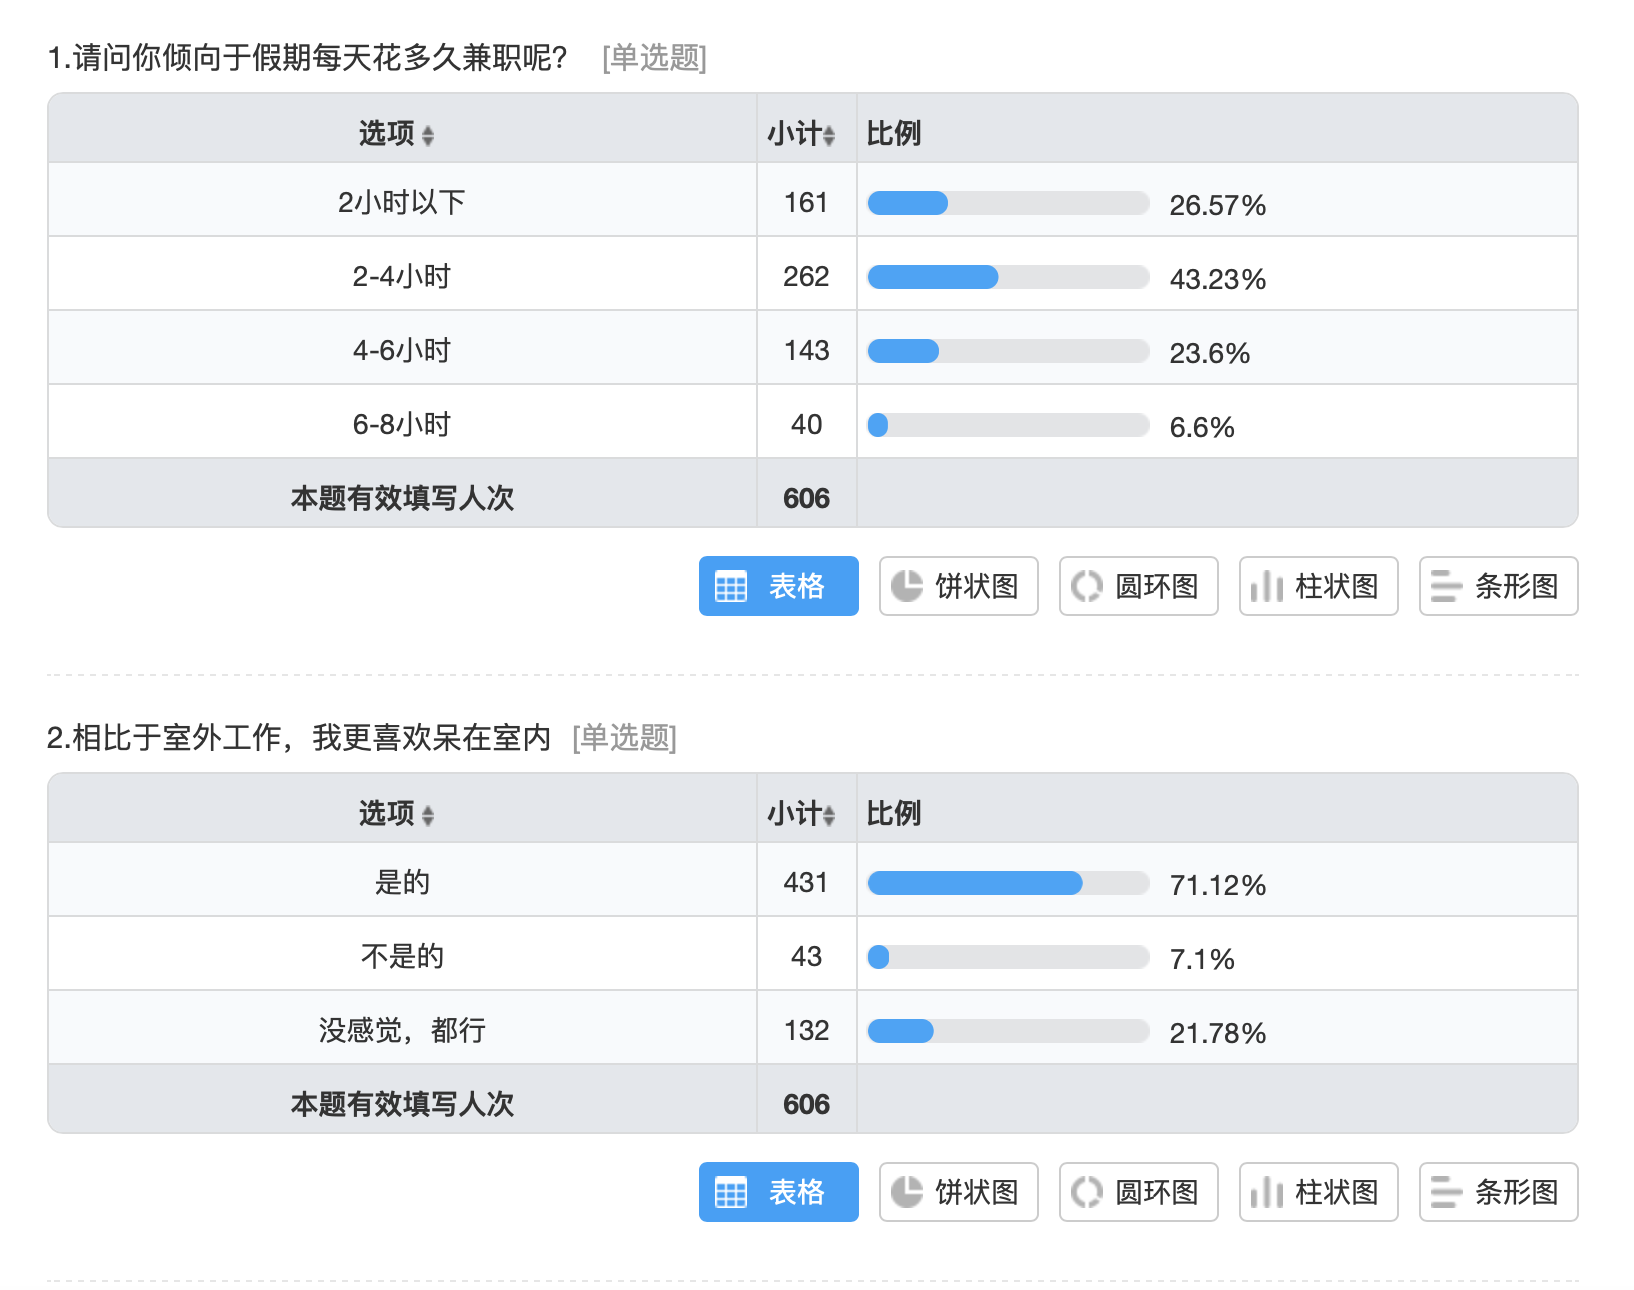
\includegraphics[width=1.7in]{figure/pic1.png}
        %\caption{fig1}
        \end{minipage}%
        }%
        % \subfigure[pic2.]
        {
        \begin{minipage}[t]{0.3\linewidth}
        \centering
        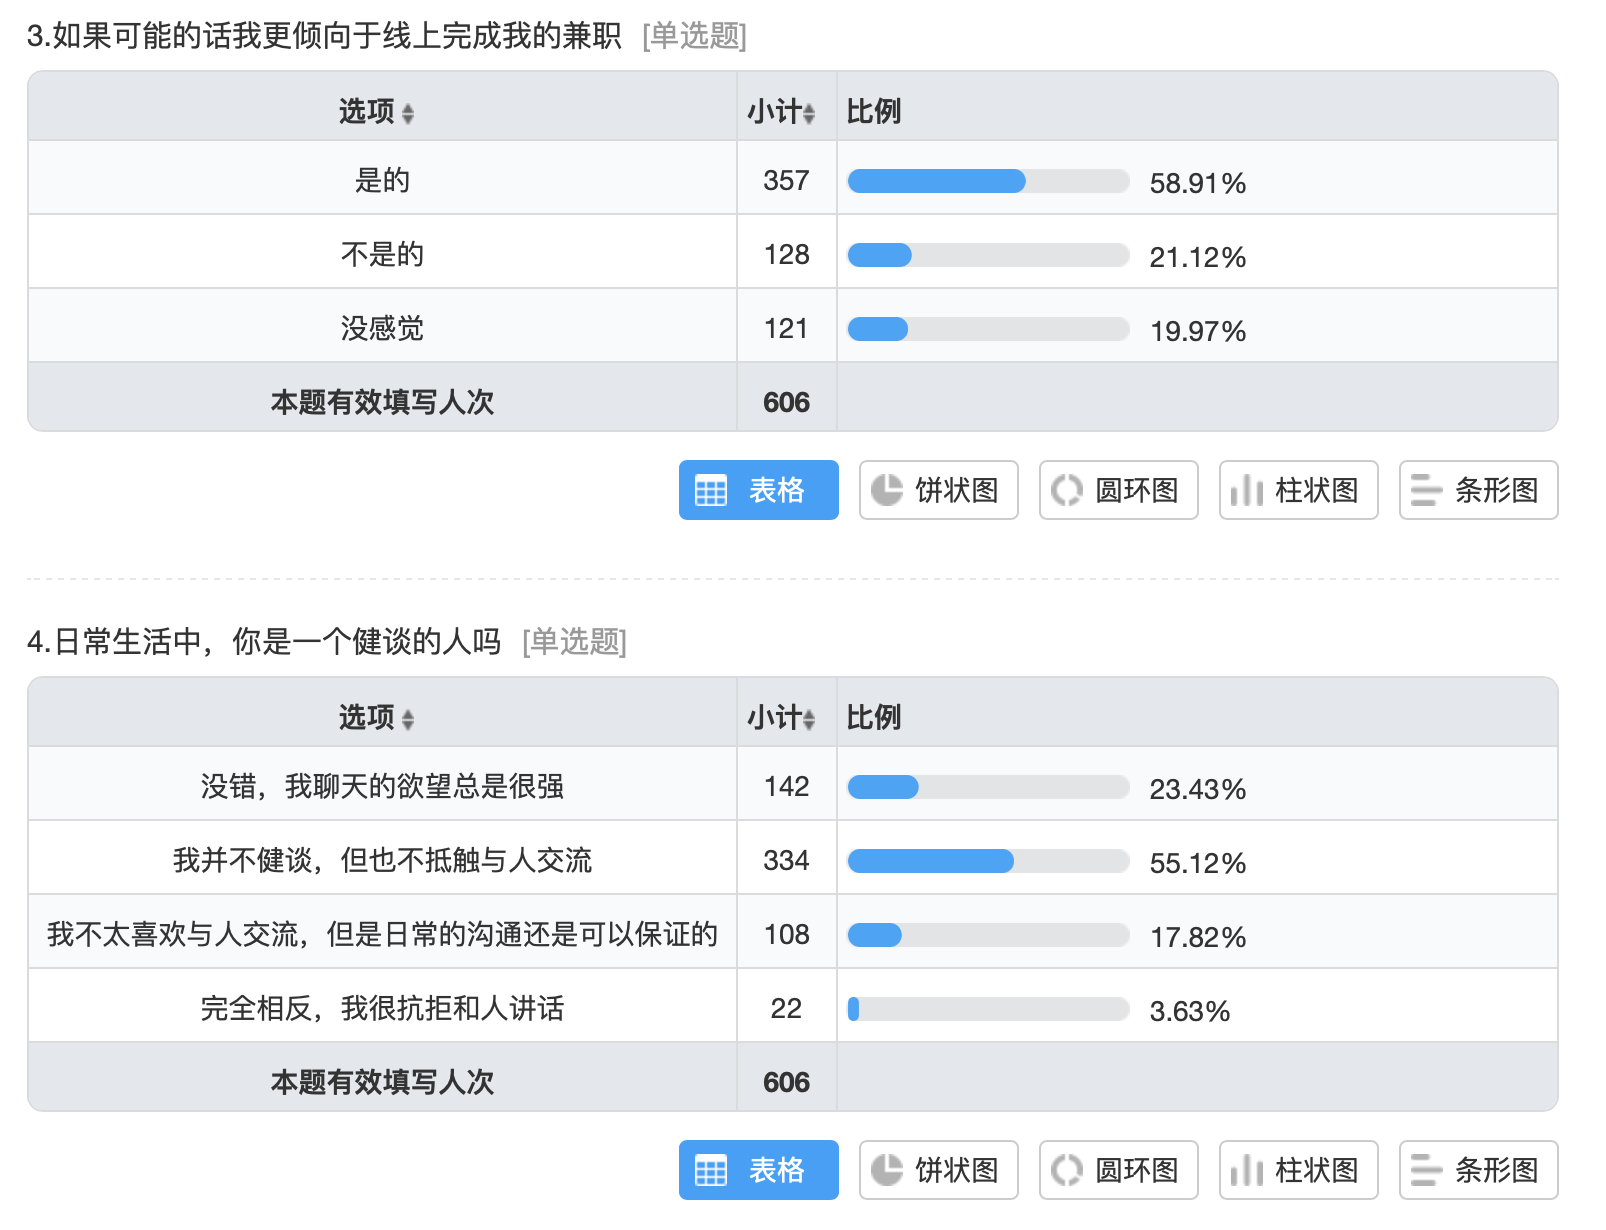
\includegraphics[width=1.7in]{figure/pic2.png}
        %\caption{fig2}
        \end{minipage}%
        }%
                         %这个回车键很重要 \quad也可以
        % \subfigure[pic3.]
        {
        \begin{minipage}[t]{0.3\linewidth}
        \centering
        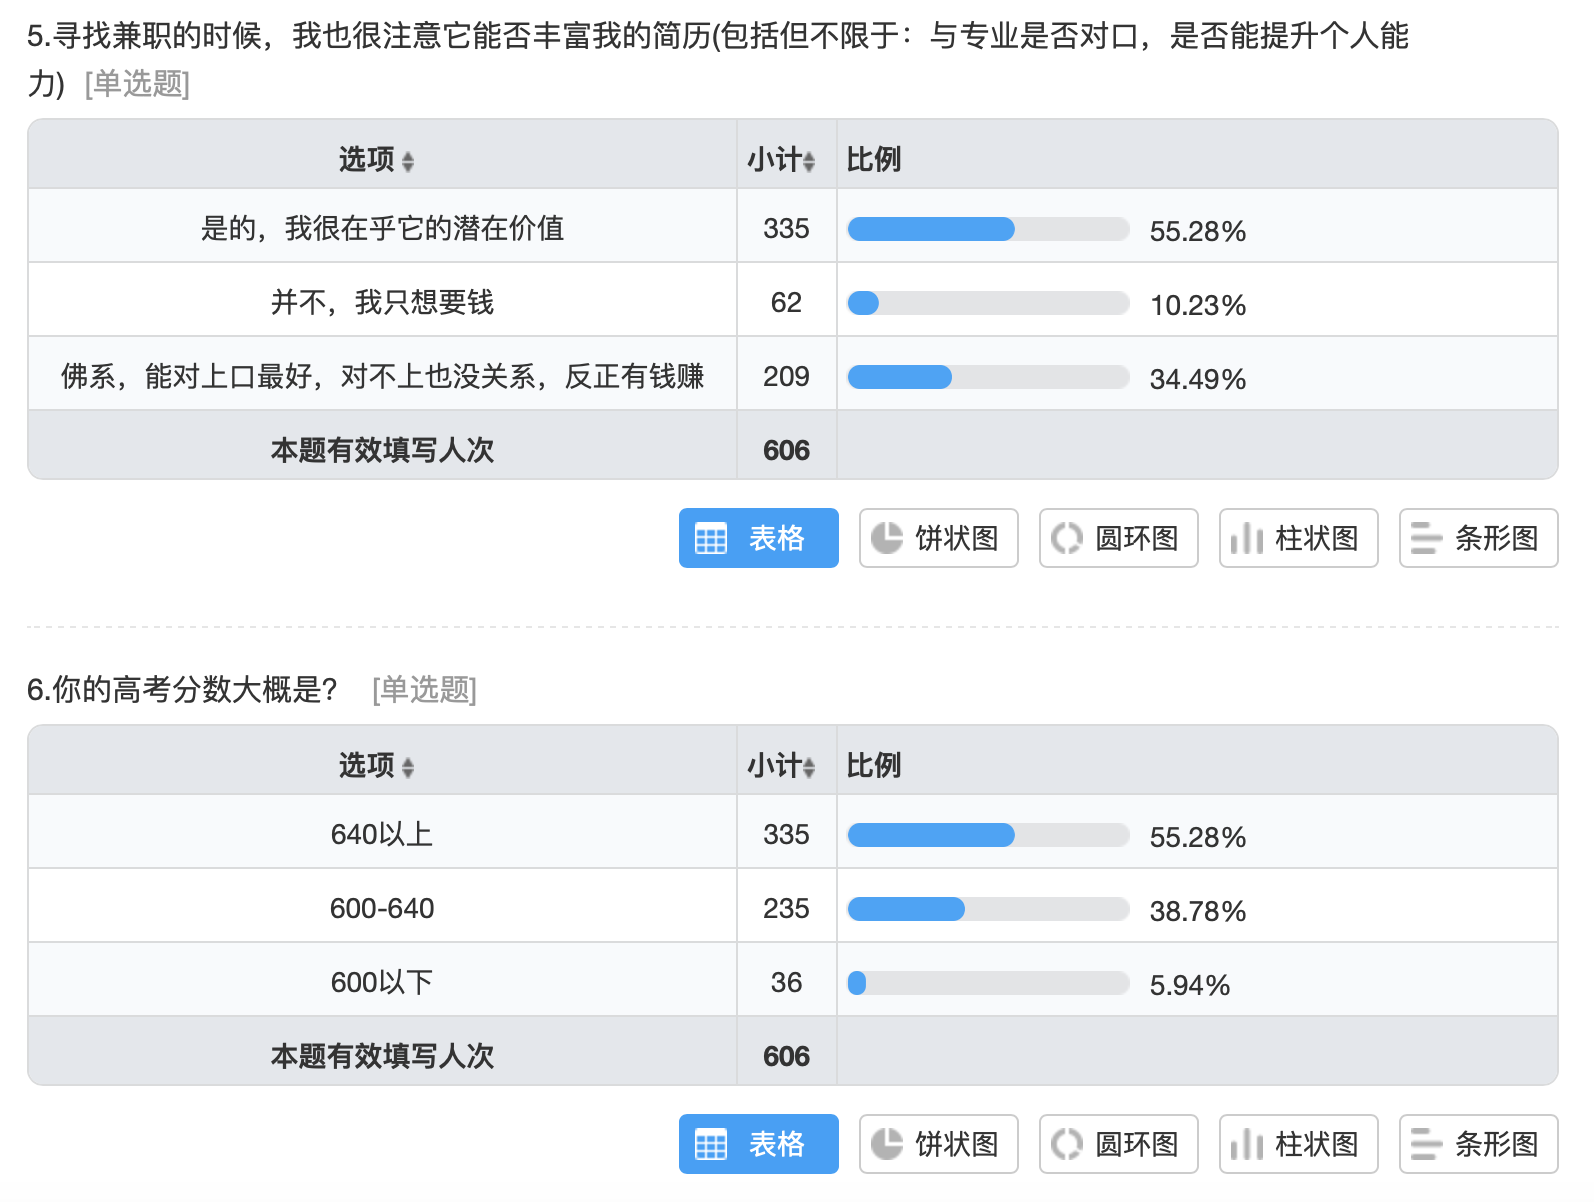
\includegraphics[width=1.7in]{figure/pic3.png}
        %\caption{fig2}
        \end{minipage}
        }%
        % \subfigure[pic4.]
        {
        \begin{minipage}[t]{0.3\linewidth}
        \centering
        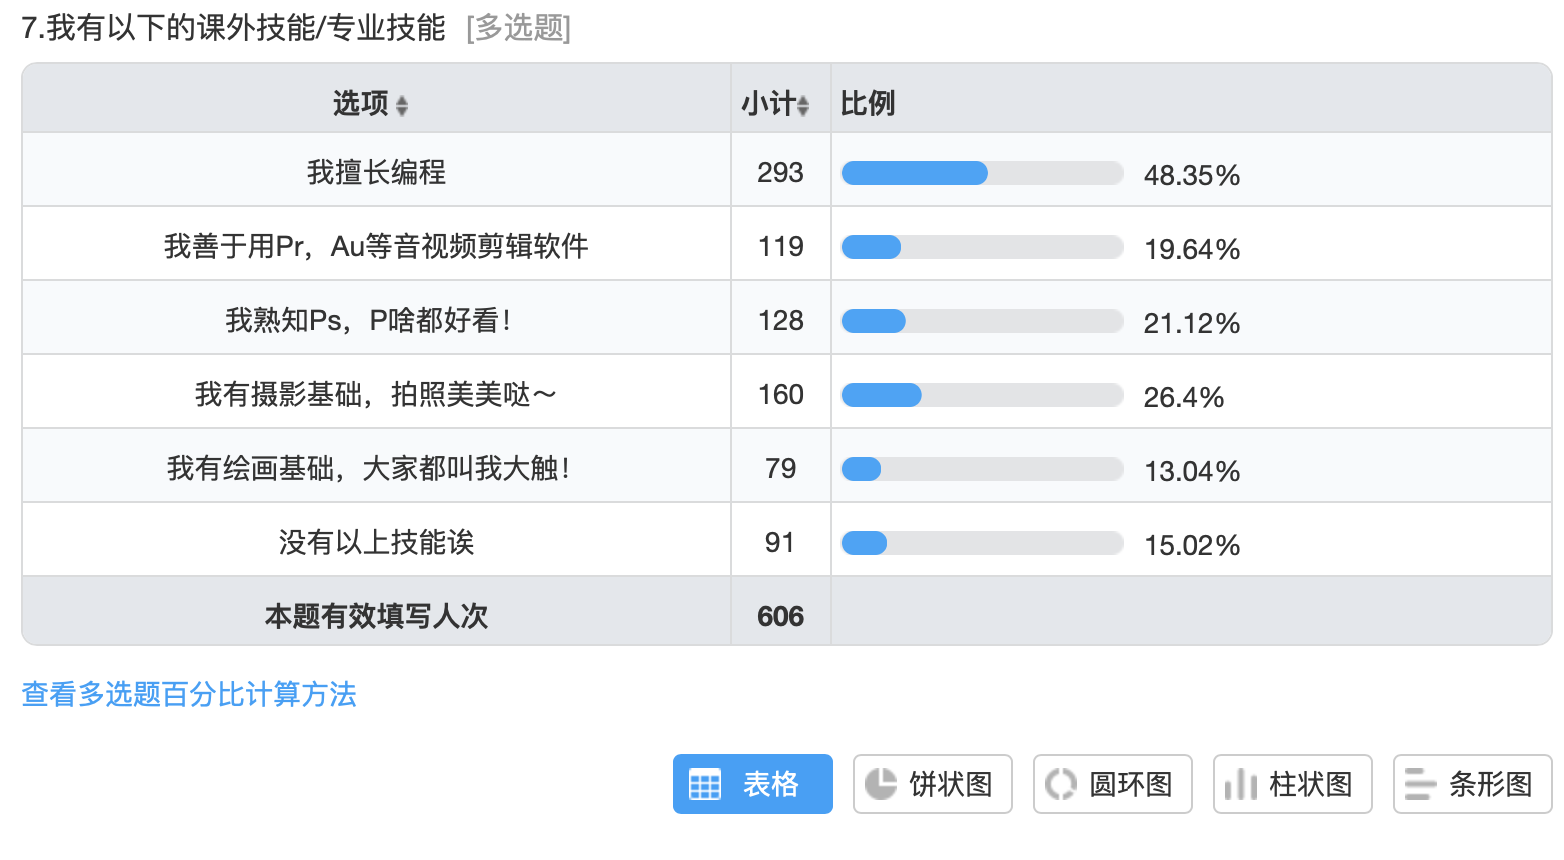
\includegraphics[width=1.7in]{figure/pic4.png}
        %\caption{fig2}
        \end{minipage}
        }%
        {
        \begin{minipage}[t]{0.3\linewidth}
        \centering
        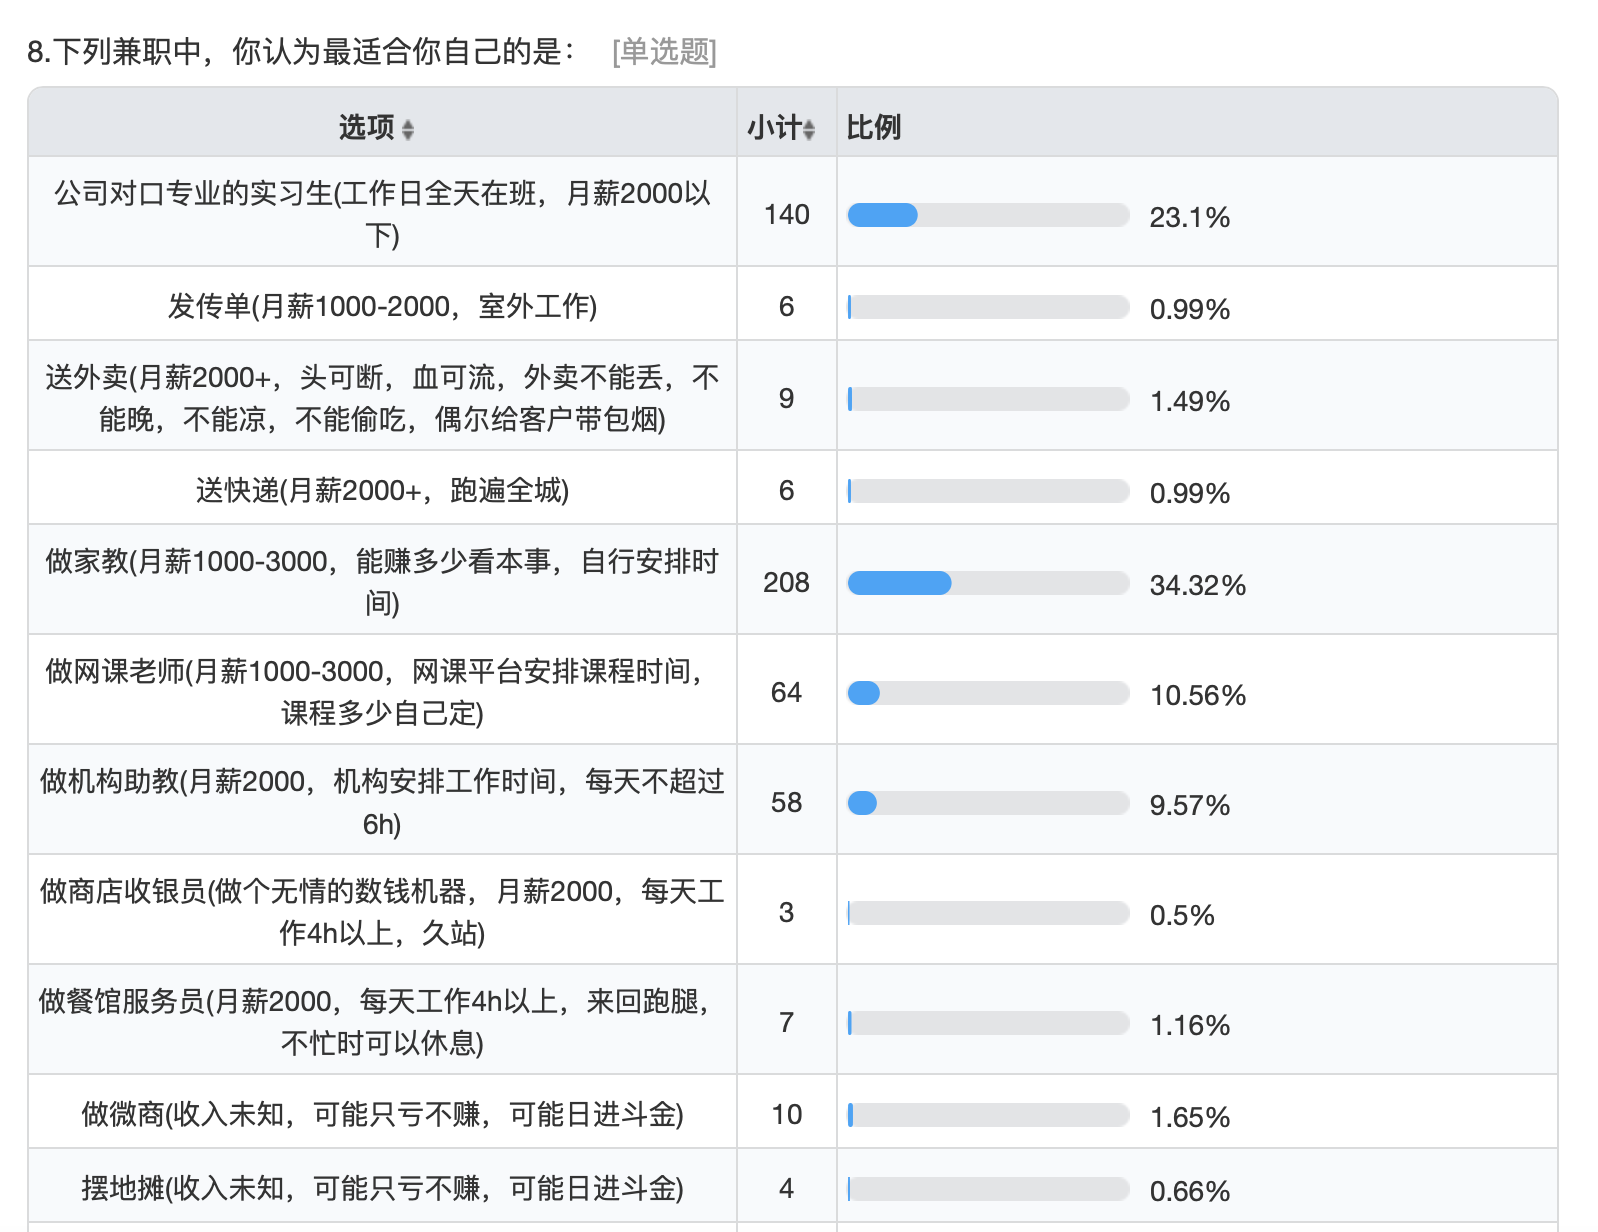
\includegraphics[width=1.7in]{figure/pic5.png}
        %\caption{fig2}
        \end{minipage}
        }
        
        % \centering
        % \caption{ pics}
        \end{figure}


    \section{Result of the Self-developed Questionnaire}
    ~~The questionnaire asks users to set limits and preferences for part-time jobs according to their own preferences.\\%这份问卷要求用户根据自身偏好对兼职工作作出限制和偏好程度的设定
    \begin{figure}[!htbp]
        \centering
        % \subfigure[pic1.]
        {
        \begin{minipage}[t]{0.3\linewidth}
        \centering
        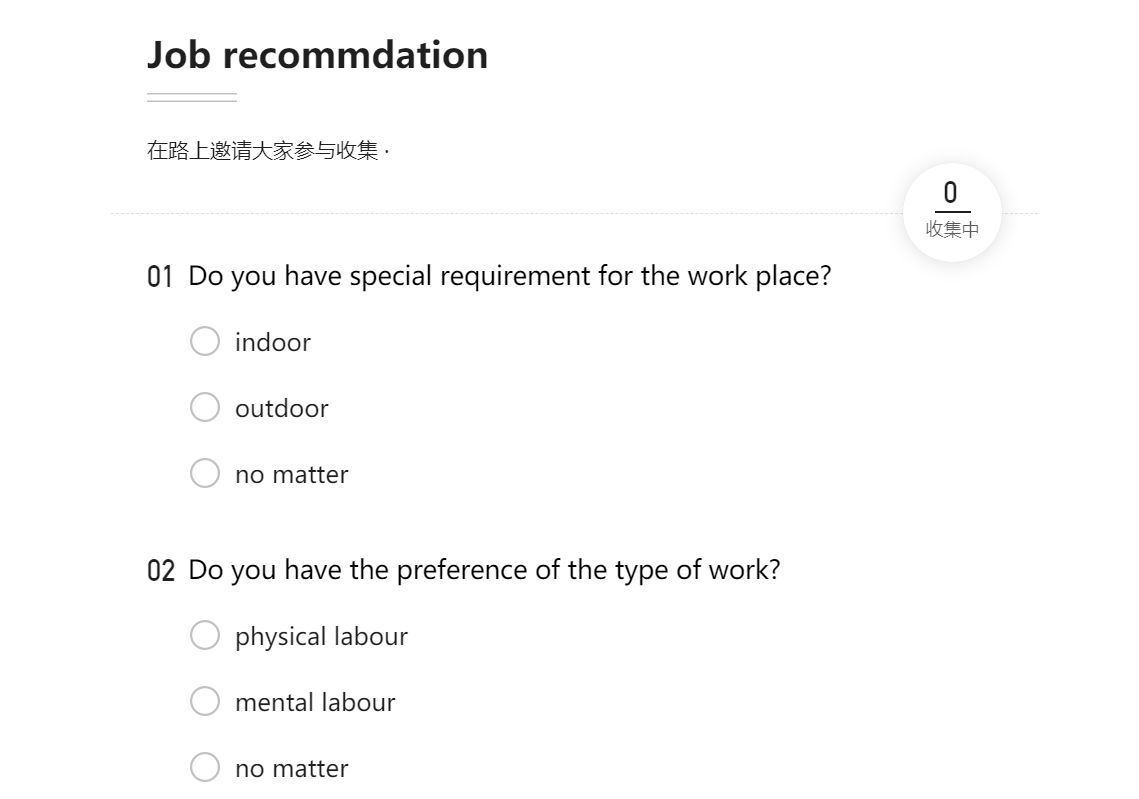
\includegraphics[width=1.7in]{figure/t1.png}
        %\caption{fig1}
        \end{minipage}%
        }%
        % \subfigure[pic2.]
        {
        \begin{minipage}[t]{0.3\linewidth}
        \centering
        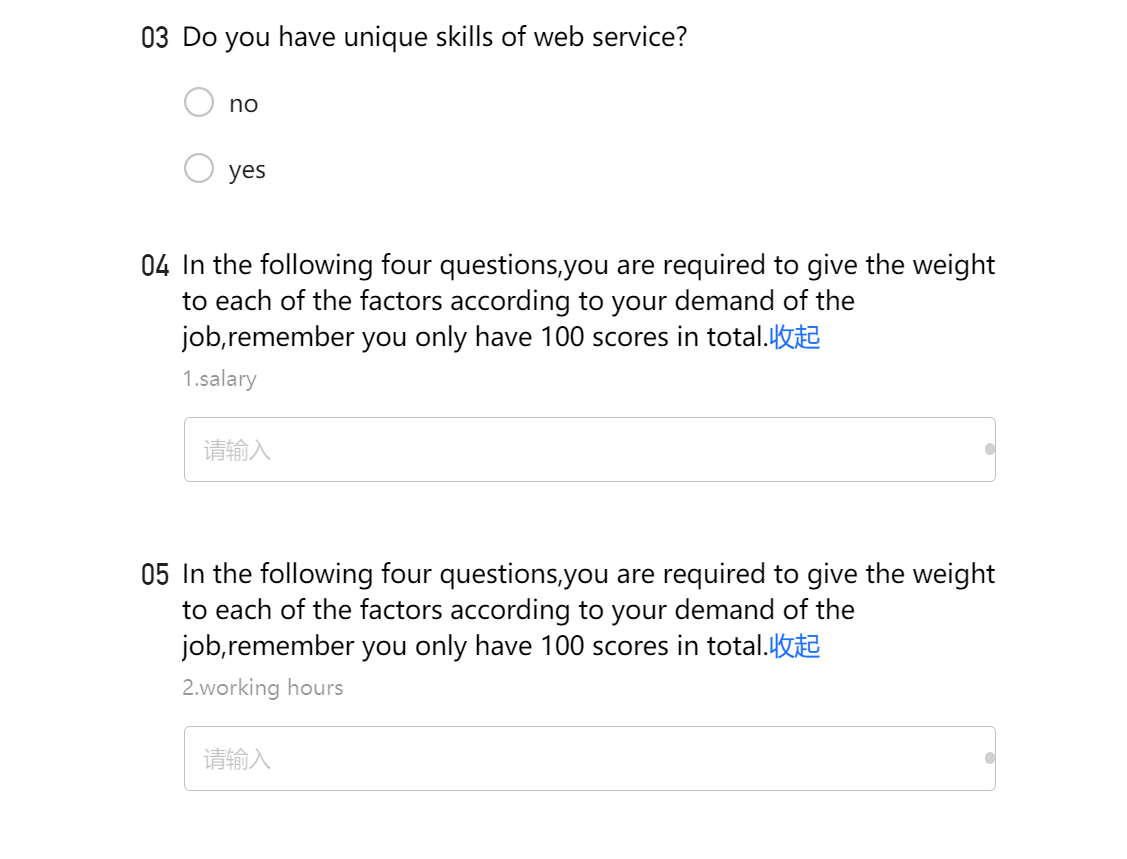
\includegraphics[width=1.7in]{figure/t2.png}
        %\caption{fig2}
        \end{minipage}%
        }%
                         %这个回车键很重要 \quad也可以
        % \subfigure[pic3.]
        {
        \begin{minipage}[t]{0.3\linewidth}
        \centering
        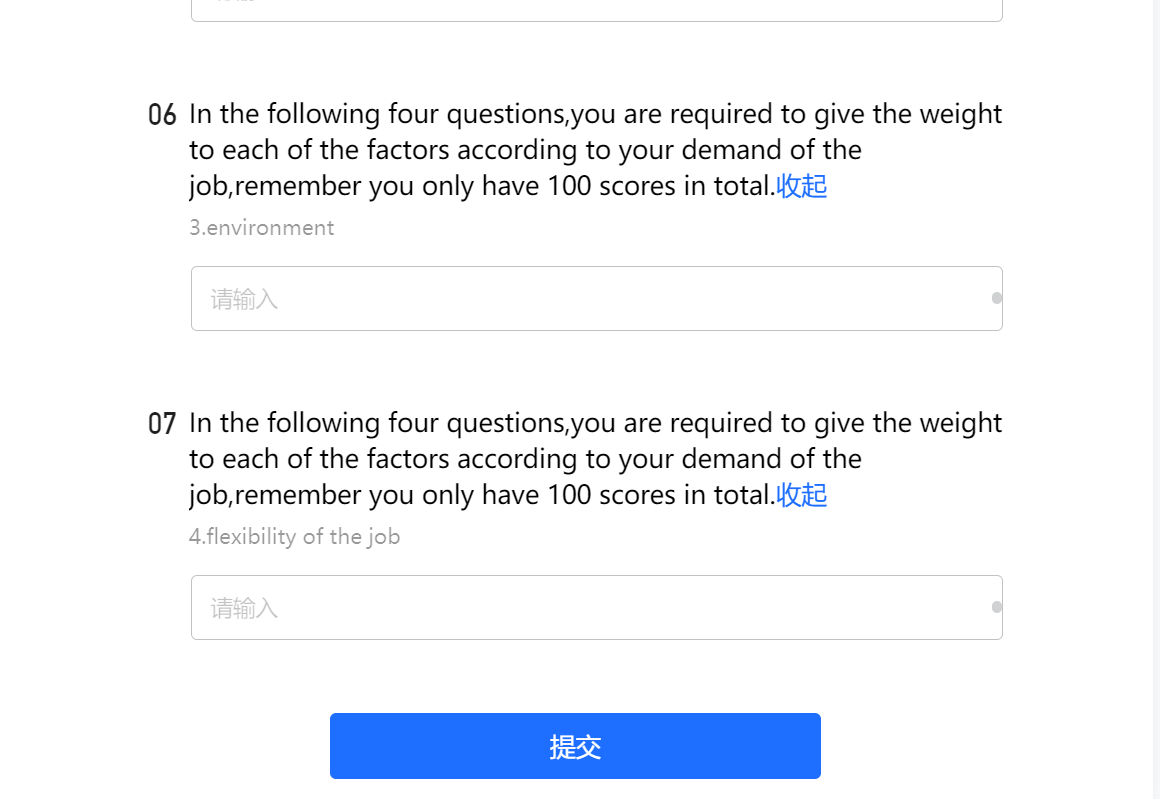
\includegraphics[width=1.7in]{figure/t3.png}
        %\caption{fig2}
        \end{minipage}
        }%
        % \subfigure[pic4.]
        \end{figure}

    \section{Source Code}
    ~~\begin{lstlisting}[language=Matlab]
        function workchoose(IN)
        work=[1.0500   -1.1670    1.0000    0.9110
            0.6280   -0.7430    1.0890    1.0000
            1.2170   -1.0610    1.1780    0.7330
            1.0000   -1.0610    0.9110    1.0890
            1.2500   -1.0610    0.7330    0.8220
            1.0500   -1.0610    0.8220    1.2670
            0.7830   -0.8490    1.2670    1.1780];
        %--------------------------------------------------------
        %When selecting a job, the proportion of each influencing 
        %factor to the corresponding job was scored

        %The rows represent the type of work and the columns 
        %represent the influencing factors

        %The types are: promotion; The waiter;Private teacher; 
        %delivery man;  workers; labor; IT workers

        %The influencing factors are as follows: salary; 
        %Working hours; The environment; flexibility
        %--------------------------------------------------------

        if IN(1,1)==1
            work(1,:)=zeros(1,4); work(4,:)=zeros(1,4);
            work(5,:)=zeros(1,4); work(6,:)=zeros(1,4);
        end
        if IN(1,1)==-1
            work(2,:)=zeros(1,4); work(3,:)=zeros(1,4);
            work(7,:)=zeros(1,4);
        end
        %---------------------------------------------------
        %Whether the multiple choice question judges indoor 
        %and outdoor work, 0== it doesn't matter;
        % 1== indoor only; -1== outdoor only
        %---------------------------------------------------

        if IN(2,1)==0
            work(5,:)=zeros(1,4); work(6,:)=zeros(1,4);
        end
        %--------------------------------------------
        %Decide whether to do labor work, 0== do not
        %--------------------------------------------

        if IN(3,1)==0
            work(7,:)=zeros(1,4);
        end
        %-----------------------------------------------------
        %Determine if you have network-related skills, 0== no
        %-----------------------------------------------------

        IN(1,:)=[]; IN(1,:)=[]; IN(1,:)=[];
        %Remove the judgment part of the questionnaire and 
        %calculate the weight

        OUT=work*IN;
        disp(OUT);
        %Calculate the output score
        NAME={'salesman','waiter','private teacher','delivery man',
        'labor','hourly worker','IT worker'};
        [R,Q]=max(OUT); OUT(Q,1)=-200;
        [R,W]=max(OUT); OUT(W,1)=-200;
        [R,E]=max(OUT);
        Result={'first choice',NAME{1,Q};
                'second choice',NAME{1,W};
                'third choice',NAME{1,E}};
        disp(Result);

        %Find and output the three jobs with the highest scores
        OUT=cell2table(Result);
        writetable(OUT,'output.txt');
        type output.txt;
        end
    \end{lstlisting}
\end{appendix}

    % \section{Results}
\end{document}






%==================sth useless=======================
% \section{承诺书}
% 我们仔细阅读了数学建模竞赛的竞赛规则.

% 我们完全明白,在竞赛开始后参赛队员不能以任何方式(包括电话、电子邮 件、网上咨询等)与队外的任何人(包括指导教师)研究、讨论与赛题有关的问题。

% 我们知道,抄袭别人的成果是违反竞赛规则的,如果引用别人的成果或其他公开的资料(包括网上查到的资料),必须按照规定的参考文献的表述方式在正文引用处和参考文献中明确列出。

% 我们郑重承诺,严格遵守竞赛规则,以保证竞赛的公正、公平性。如有违反竞赛规则的行为,我们将受到严肃处理。

% 我们的题目编号是:\dlmu[5.75cm]{A}

% 队号:\dlmu[8cm]{H275}

% 参赛队员姓名学号(中文填写打印并签名):

% \begin{enumerate}
%     \item \dlmu[9cm]{~王大杨2019021404012~}
%     % \underline{\hbox to 9cm{~王大杨2019xxxxxxxxx~}}
%     \item \dlmu[9cm]{~陈麒至2019091601015~}
%     \item \dlmu[9cm]{~王泽寰2019021404008~}
% \end{enumerate}


% \section{Reference}%引用时使用:\cite{ref1,ref2,...}
% \begin{thebibliography}{99}  
%     \bibitem{ref1} 
%     \bibitem{ref2} 
%     \bibitem{ref3}
%     \bibitem{ref4} 
% \end{thebibliography}